%!TEX root=../book.tex

\chapter{\textit{t}-Tools}

\section{Overview of \textit{t}-Tools}

\subsection{One-Sample \textit{t}-tools}

The one-sample \textit{t}-test is one of the simplest entry points to inferential statistics there is. Simply put, it seeks to determine if the average value of a set of data differs significantly from some theoretical quantity. Say, for instance, we are working in a lumber mill and it looks like a shipment of Douglas fir trees is a bit smaller than usual. We know that a typical Douglas fir from this region is about 225 feet tall and has a radius of 7.5 feet, giving us a total volume of about $39000$ cubic feet.

So we take the measurements for each of the trees in this shipment and find that the average volume is $36500$ cubic feet with a standard deviation around $\sigma = 2000$ cubic feet. Do we have sufficient proof that these trees are actually smaller than our typical shipment?

Well, unfortunately, the human brain isn't great at intuitively figuring out if differences like that are meaningful or within the expected margin of error: that's where inferential statistics come into play. So let's first state our hypotheses as:
\begin{eqnarray*}
H_0:& \bar{x} = \mu\\
H_A:& \bar{x} \neq \mu
\end{eqnarray*}
where $\bar{x}$ is the mean volume of our shipment of trees and $\mu$ is the mean volume of adult Douglas firs. Now, we can conduct our statistical test.

A \textit{t}-test, speaking generally, takes the form:
\begin{equation}
t = \frac{\text{Estimate}-\text{Parameter}}{SE(\text{Estimate})}
\end{equation}
The specifics of what you plug in for the estimate and the parameter will vary a bit depending on which type of \textit{t}-test you use; however, they all are based off of this.

In our case, the one-sample \textit{t}-test will look like:
\begin{equation}
t=\frac{\bar{x}-\mu}{se_x}
\end{equation}
where each of the variables is what we defined in our hypotheses above. Plugging in our data we get:
\begin{eqnarray*}
t(124)&=&\frac{36500-39000}{2000/\sqrt{125}} \\
&=& -13.98
\end{eqnarray*}
Although we have our standardized \textit{t}-statistic, we still don't know if it reaches a level of significance or not. historically, we would have to go to a table of \textit{p}-values and look up the one that was closest to our \textit{t}-statistic given the degrees of freedom (here, 124, or $n-1$). Thankfully, we now have software that is able to compute this value for us much more precisely and quickly. In this case, we end up with a \textit{p}-value $< 0.001$, showing that the result is highly significant.

Moreover, we can infer the direction of this difference. Remember that the \textit{t}-statistic is computed by subtracting our estimated mean from our population mean: given this, a negative \textit{t}-statistic means that the sample mean is less than the population mean whereas a positive \textit{t}-statistic shows that our sample mean is greater than that of the population.

So, we can ultimately conclude that this shipment of Douglas firs is statistically significantly below the average size of a shipment, given $t(124)=-13.98$ with a $p\text{-value} < 0.001$. We can summarize this difference in Figure \ref{fig:t01}.

\begin{figure}[h]
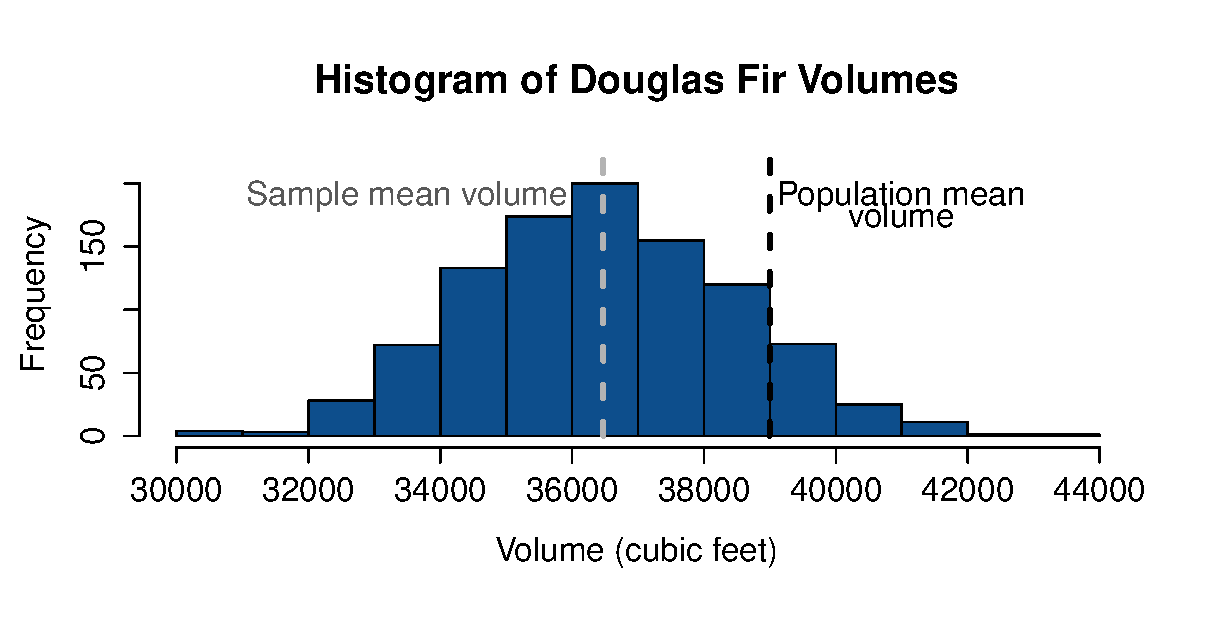
\includegraphics[width=35pc]{t01}
\label{fig:t01}
\caption{Histogram of the volumes of a shipment of Douglas firs with mean volume $36500$ cubic feet and standard deviation $\sigma = 2000$ cubic feet. A one-sample \textit{t}-test shows that this shipment of firs is significantly smaller than the typical shipment (mean $39000$ cubic feet), $t=-13.98$, $p\text{-value}<0.001$.}
\end{figure}

\subsection{Paired-Samples \textit{t}-Tools}

So now that we're familiar with a one-sample \textit{t}-test, the next two tests in the suite become really easy to understand. In a one-sample \textit{t}-test, we're testing one sample of data against a mean that we already know. I

\begin{figure}[h]
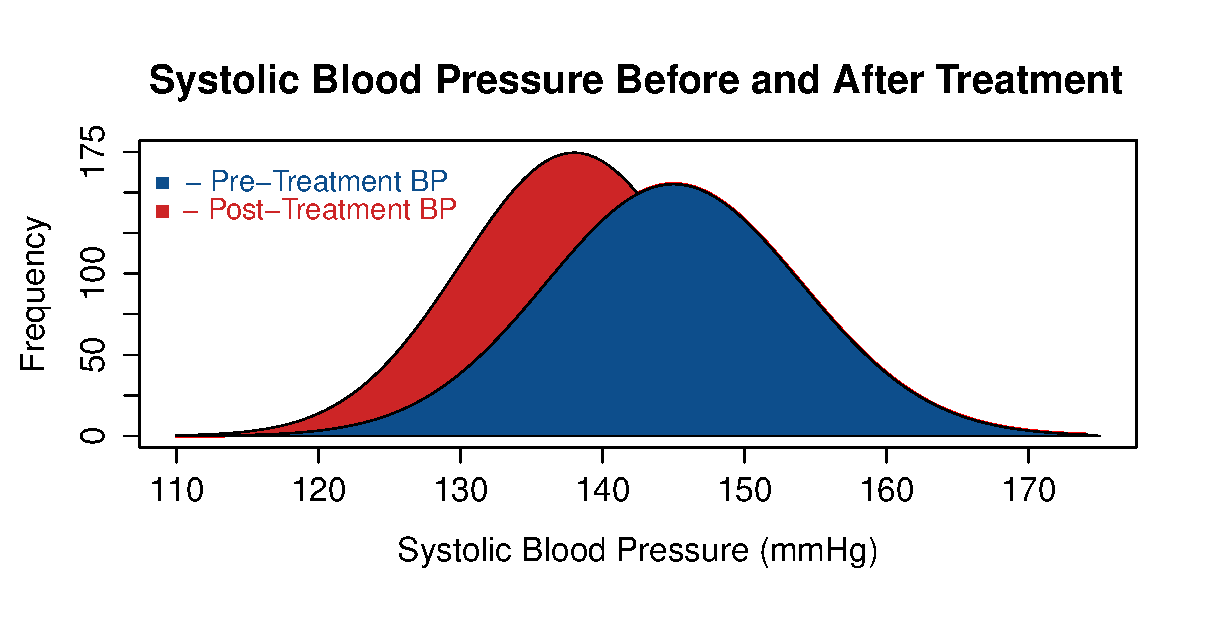
\includegraphics[width=35pc]{t02}
\label{fig:t02}
\caption{The distributions of two shipments of logs from two different logging sites.}
\end{figure}

\subsection{Independent-Samples \textit{t}-Tools}

\section{Cautions and Considerations}

\subsection{Assumptions}

\subsection{Equality of Variances}

\subsection{Robustness of \textit{t}-Tools}

\subsection{Resistance to Outliers}

\section{Implementation in R}

\section{Case Study: [STUDY]}

\section{Exercises}

\section{Additional Resources}
